\documentclass[a4paper]{article}

\usepackage[ngerman]{babel}
\usepackage[normalem]{ulem}
\usepackage[utf8]{inputenc}
\usepackage{graphicx}

\title{Bachelor Arbeit Proposal\\
  Detailliertere Beweisgenerierung in SMTInterpol
}
\author{Markus Pomrehn\\{markus.pomrehn@gmail.com}}
\date{\today}

\begin{document}

\maketitle

\section{Zusammenfassung}

Da der momentane Prooftracker, der den Beweis für die Umformung einer Eingabeformel erst in eine äquivalente Negation Normal Form (NNF) und dann in eine erfüllbarkeitsäquivalente Konjunktive Normal Form (KNF), mitschreibt, einige Probleme hat, soll dieser umgeschrieben werden.
Die Umformung in NNF wird nach De Morgan's Laws gemacht und vom Termcompiler ausgeführt.
Die Umformung in KNF wird nach Plaisted und Greenbaum gemacht und vom Clausifier ausgeführt.
Die generierten Beweise sind schwer zu lesen und in einigen Fällen sogar falsch.
Außerdem sind die Beweisregeln aufwendig zu prüfen, für jede Ersetzungsregel muss die gesamte Formel durchlaufen werden.
Aufwand $O(n^2)$, statt $O(n)$. Diese Probleme sollen mit neuen Umschreiberegeln angegangen werden.

\section{Aufgabenbeschreibung}

Zuerst muss der Prooftracker angepasst, bzw. erweitert werden um die Regeln Reflexivität, Transitivität und Kongruenz.
Ziel ist es jeden Umschreibeschritt genau zu dokumentieren.
Dann muss der Termcompiler so angepasst werden, das er die neuen Regeln verwendet.
Und zuletzt muss der Clausifier angepasst werden, im speziellen die Methoden addAsAxiom und addAxiom.

\section{Arbeitspakete}

\subsection{Einarbeitung}

Zuerst muss man sich mit dem vorhandenen Beweisverfahren auseinander setzen, beziehungsweise es verstehen.
Nachvollziehen, wie die beteiligten Klassen mit einander arbeiten.
Dazu den Programm Code heran ziehen.

\paragraph{Ergebnis:}
Möglichst vollständiges Verständnis vom Code.
Teil des Kapitels Beweisformat Alt.
Kapitel: Implementation Alt.

\subsection{Neues Beweisformat}

Zu den vorhandenen Beweisregeln sollen die oben erwähnten Reflexivität, Transitivität und Kongruenz hinzugefügt werden.

\paragraph{Ergebnis:}
Teil des Kapitels Beweisformat Neu.
Teil des Kapitels Entwurf (Beispiel Beweisgenerierung)


\subsection{Implementierung Prooftracker}

\paragraph{Prooftracker umschreiben}

Hinzufügen der neuen Beweisregeln.

\paragraph{TermCompiler anpassen}

Verwendung der dem Prooftracker hinzugefügten Regeln hinzufügen.

\paragraph{Clausifier anpassen}

Die Methoden addAsAxiom und addAxiom anpassen.

\paragraph{Ergebnis:}
Kapitel Entwurf fertig, Kapitel Implementierung, Implementierung fertig

\subsection{Test und Evaluierung}

So früh wie möglich sollte mit Testen begonnen werden.
Sobald dem Prooftracker die Regeln hinzugefügt wurden, sollten diese auch getestet werden.
Das Testen läuft parallel zu Implementierung.
Bei der Evaluierung die Beweise auf Lesbarkeit, Korrektheit und Geschwindigkeit bei der Erstellung untersuchen.

\paragraph{Ergebnis:}
Testfälle, Statistiken,
Kapitel Evaluierung in der Bachelorarbeit.

\subsection{Bachelorarbeit aufschreiben}

Auch das Aufschreiben so früh wie möglich beginnen.
Zu den bisher erwähnten Teilen der Bachelorarbeit Einführung, Fazit hinzufügen und am Ende auf 
Rechtschreibfehler prüfen.

\paragraph{Ergebnis:}
Die fertige Bachelorarbeit


\section{Zeitplan}

Für jedes Arbeitspaket eine Angabe der Dauer (in Wochen).
Gantt Diagramm

\centerline{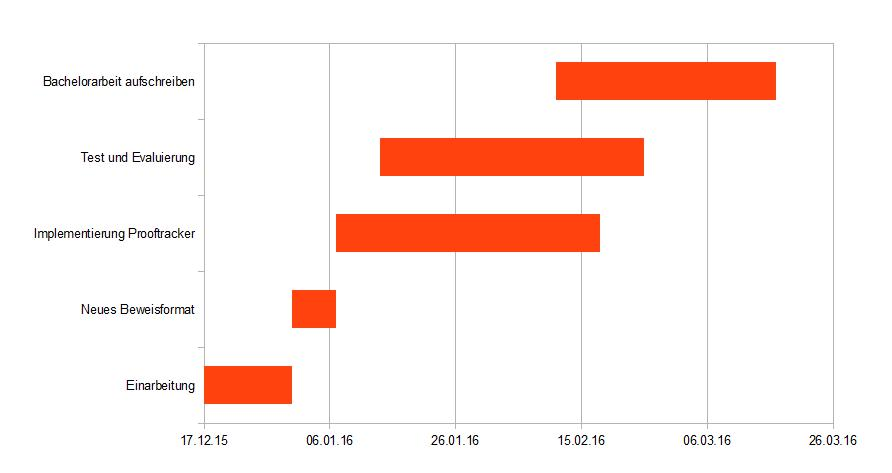
\includegraphics[scale=0.5]{Ganttchart}}


\bibliography{references}

\end{document}
